\documentclass[runningheads]{llncs}
%
\renewcommand{\figurename}{Figure}

\usepackage[T1]{fontenc}
\usepackage{graphicx}
\usepackage{amsmath}
\usepackage{amssymb}
\usepackage{float}
\usepackage{multirow}
\usepackage{booktabs}
\usepackage{marvosym}
\usepackage{ifsym}
\usepackage[table]{xcolor}
\usepackage{placeins}
\usepackage{xcolor}
\usepackage{indentfirst} % indent the first paragraph after every heading too, for uniform paragraph indentation
\usepackage[autostyle=false, style=english]{csquotes}\MakeOuterQuote{"}

% hyperref must be loaded last; makes \cite, \ref and URLs clickable
\usepackage{hyperref}
\hypersetup{
  colorlinks=true,
  linkcolor={black},
  citecolor={black},
  urlcolor={black}
}

\renewcommand{\arraystretch}{1.1}

% Standard LaTeX float parameters, so floats sit near their reference
\renewcommand{\topfraction}{0.9}
\renewcommand{\bottomfraction}{0.7}
\renewcommand{\textfraction}{0.1}
\renewcommand{\floatpagefraction}{0.8}

\graphicspath{{figures/}}

% LNAI: no colour in text/tables/equations. "best" = bold black (matches captions).
\newcommand{\best}[1]{\textbf{#1}}

\begin{document}
%
\title{A Two-Branch Hybrid Model for Imbalanced Lumbar Disc Grading and Zero-Shot Label Extension}
%
\titlerunning{A Two-Branch Hybrid Model for Lumbar Disc Grading}
%
% ----- CAMERA-READY author block (MIWAI 2026) -----
\author{Trung Kien Ha\inst{1,2} \and
Trong Nhan Phan\inst{1,2}\textsuperscript{(\Letter)}}
\authorrunning{T. K. Ha and T. N. Phan}
\institute{Faculty of Computer Science and Engineering, Ho Chi Minh City University of Technology (HCMUT), 268 Ly Thuong Kiet, Dien Hong Ward, Ho Chi Minh City, Vietnam.
\and
Vietnam National University Ho Chi Minh City (VNU-HCM), Linh Xuan Ward, Ho Chi Minh City, Vietnam.\\
\email{\{htkien.sdh242,nhanpt\}@hcmut.edu.vn}}
%
\maketitle
%
\begin{abstract}
Automated grading of lumbar intervertebral disc (IVD) pathology on MRI is clinically useful but hard: severity classes are heavily imbalanced, large labelled volumetric datasets are scarce, and a model trained on one labelling schema cannot answer a query posed in another schema without retraining a new classifier head. We address these problems by design rather than by a single component. We propose a two-branch model in which a volumetric attention branch captures cross-slice anatomical context and a frozen multimodal (vision-language) branch supplies a semantic prior learned from large-scale biomedical pretraining; then a small trainable head fuses the two streams into a text-aligned embedding. Because predictions are made by matching this embedding to text prompts, the label set becomes an input to inference, so the same trained model can grade a new label set with no extra head and no retraining. We implement the two branches with a CBAM-equipped 3D ResNet-34 and a frozen BiomedCLIP encoder, and we validate the design on the RSNA 2024 and SPIDER datasets. With focal loss, square-root class weighting, minority oversampling, and standard augmentation, the model raises Severe-class recall from 12.3\% to 48.6\% and Severe F1 from 0.152 to 0.356 on RSNA 2024. Without any fine-tuning it extends to eight unseen SPIDER labels through text prompts (mean F1 = 0.362), and under supervised transfer it matches SpineNetV2 on aggregate SPIDER F1 ($0.653$ vs.\ $0.646$) while exceeding the attention-only variant by $+0.034$ (paired $t$-test, $p=0.011$), which suggests the frozen branch helps regularize cross-dataset transfer.

\keywords{spine MRI \and intervertebral disc grading \and attention \and vision-language models \and BiomedCLIP \and zero-shot classification \and class imbalance \and low back pain}
\end{abstract}
%
%==============================================%
\section{Introduction}\label{sec1}

Low back pain is the leading cause of disability worldwide, and lumbar disc degeneration drives most interventions that follow. Quantitative MRI grading of intervertebral disc (IVD) pathology (spinal canal stenosis, left and right neural foraminal stenosis, Pfirrmann grade) is still largely manual and carries substantial inter-rater variability~\cite{nigru2024}. Automated 3D convolutional systems such as SpineNet~\cite{jamaludin2017} and SpineNetV2~\cite{windsor2022} have made real progress, yet two problems remain open. First, class imbalance: the most important class (Severe) is usually under 5\% of training samples, and ordinary cross-entropy training all but ignores it, with Severe recall near zero. Second, a fixed label space: a model trained on one schema (e.g.\ the 3-condition $\times$ 3-severity grid of RSNA 2024~\cite{kaggle2024}) cannot answer a query phrased in another (e.g.\ the Pfirrmann, spondylolisthesis, and herniation labels of SPIDER~\cite{vandergraaf2024spider}) without retraining a new fixed-class head.

The two gaps share a cause: trained from scratch on a single dataset, existing graders overfit its minority-class statistics and lock in a fixed head, so accuracy drops on a new center and a new label schema needs a retrained head. We address both by design. For imbalance, we anchor the volumetric encoder with a \emph{frozen biomedical foundation model}~\cite{zhang2023biomedclip}, whose large-scale pretraining gives a stable prior where Severe examples are too scarce to learn from scratch, and we add channel-spatial attention~\cite{woo2018cbam} to focus on the small region a Severe lesion occupies. For the fixed label space, we exploit the same model's shared image-text embedding~\cite{radford2021clip}, which lets a new label set enter inference as a text prompt instead of a retrained classifier head. These two ideas form the two branches of our model, joined by a small trainable fusion head, whose details are given in Section~\ref{sec3}. In general, our main contributions are as follows.
\begin{itemize}
    \item \textbf{A cross-dataset transfer finding.} Channel-spatial attention helps the rare Severe class when the model is tested on the dataset it was trained on (RSNA), but that benefit disappears on a different dataset (SPIDER). Adding the frozen multimodal branch brings the benefit back and keeps performance stable across datasets ($+0.034$ in mean F1 over attention alone); the frozen branch appears to stop attention from over-fitting to a single dataset.
    \item \textbf{A complementary two-branch design.} We couple a volumetric attention encoder~\cite{woo2018cbam} with a frozen multimodal prior~\cite{zhang2023biomedclip} through a small learned fusion; an ablation shows the two branches are complementary rather than redundant.
    \item \textbf{Label-space extension without retraining.} Because labels are scored by matching the image embedding to text prompts, the label set becomes an input to inference: the same trained model can score a prompt-defined target label schema with no new classifier head and no retraining, unlike fixed-head baselines. Section~\ref{sec4} instantiates this with RSNA as source and SPIDER as a held-out target schema.
    \item \textbf{A training pipeline that recovers the minority class.} An imbalance recipe (focal loss~\cite{lin2017focal}, square-root class weighting, minority oversampling, augmentation) combined with the two-branch architecture raises the near-zero Severe recall of cross-entropy training about $4\times$ (12.3\% to 48.6\%) on RSNA 2024.
\end{itemize}

The rest of the paper covers related work (Section~\ref{sec2}), the task formulation and two-branch model (Section~\ref{sec3}), RSNA and SPIDER results (Section~\ref{sec4}), and discussion and conclusions (Sections~\ref{sec:disc}--\ref{sec5}).

%==============================================%
\section{Related Work}\label{sec2}

Automated disc grading began with SpineNet~\cite{jamaludin2017}. It takes one intervertebral disc volume as input, is trained only on disc-specific labels, and predicts several radiological gradings at once, together with hotspot maps showing where the evidence lies. It was developed on the GENODISC corpus of lumbar T2 scans. Windsor et al.~\cite{windsor2022} later released SpineNetV2, an open-source pipeline that detects vertebral bodies, labels the levels, and then grades each disc. It crops one volume per disc and resamples it to $112\times224\times9$, the input format we reuse unchanged. Its grading network covers eight schemes with a single shared model, including Pfirrmann, disc narrowing, central canal stenosis, and several binary findings. The eight schemes are fixed before training, so a ninth one needs a new output head and new training. Clinically validated graders reach near-radiologist agreement on stenosis grading~\cite{hallinan2021}, while external validations report a foraminal F1 near 0.84 at a balanced accuracy of about 0.69 to 0.70~\cite{mcsweeney2023,nigru2024}, reflecting the lower ceiling of sagittal-only foraminal reads. We reuse the SpineNetV2 3D ResNet grading backbone (one volumetric crop per disc) so its pretrained weights transfer without modification.

None of these systems targets the heavily skewed three-class severity setting we study, where the Severe class falls below 5\% of samples. The usual remedy is channel-spatial attention. The CBAM block~\cite{woo2018cbam} refines a feature map twice: first it reweights the channels, then it reweights the spatial positions. It is small, can be inserted after any convolutional stage, and was designed for 2D images. It has since been used for lumbar stenosis classification~\cite{lin2024cbam}. We extend it to a fully 3D form so that both steps also see the sagittal dimension. Attention sharpens where the model looks, but it does not change which labels the model can answer. Because we keep the harder full three-class grading on its native imbalanced distribution and score one model with macro metrics, our numbers are not directly comparable to the differently-posed published RSNA~2024 solutions, whether joint segmentation-and-classification~\cite{aktan2025}, ensemble log-loss~\cite{kaggle2024}, or open pipelines~\cite{nshen2024}. Crucially, all of these train a fixed classifier head on a single schema and cannot take a new label set as input, the gap our prompt-based design fills.


BiomedCLIP~\cite{zhang2023biomedclip} trains a CLIP-style~\cite{radford2021clip} image-text model on PMC-15M (fifteen million figure-caption pairs from PubMed Central). The benchmark of Woerner and Baumgartner~\cite{datascarcity2024} shows its linear probe overtaking supervised training when labels are few (exactly the regime of our Severe class), which is why we use it frozen rather than fine-tuned. The closest architecture is RadCLIP~\cite{lu2024radclip}. It keeps the CLIP two-encoder design and adds a slice-pooling adapter that merges 2D slice features into one volume-level vector, so no 3D convolution is needed. Its image encoder is fine-tuned against a frozen text encoder with a contrastive loss. The closest application is LumbarCLIP~\cite{le2025lumbarclip}, a CLIP-style model trained from scratch on lumbar MRI paired with expert reports, which reports up to 95.00\% accuracy on its own classification task. Both need paired image and text data from the target domain, and both are tested on the schema they were trained for. We differ from both: BiomedCLIP stays frozen and we read its text-aligned embedding by cosine similarity, so the same model answers a new label set zero-shot by swapping prompts, studying cross-dataset label-space extension rather than in-distribution accuracy. The head is parameter-free rather than prompt-tuned; native 3D medical vision-language models are a natural future backbone, and controlled comparisons with newer medical vision-language backbones are left to future work.

%==============================================%
\section{Proposed Method}\label{sec3}

\subsection{Problem Formulation}\label{sec:formulation}

We state the grading task and its zero-shot extension in one notation. Let $\mathcal{V}$ be the space of per-IVD volumetric crops (concrete dimensions in Section~\ref{exp1}). A grading model is a composition
\begin{equation}
h = c \circ \Phi,
\label{eq:composition}
\end{equation}
where the shared encoder $\Phi:\mathcal{V}\to\mathbb{R}^{d}$ maps a volume to an embedding $f=\Phi(v)$ of dimension $d$, and the head $c$ turns it into class probabilities over a label set $\mathcal{Y}$. The head $c$ is a linear head for the baselines and a prompt-based cosine head for the Multimodal-only and Hybrid configurations; for the latter, zero-shot extension keeps the head and all learned weights fixed and only swaps the prompt-defined label set $\mathcal{Y}$.

In the supervised setting, the fixed-head baselines (SpineNetV2, CBAM-only) use a linear head
\begin{equation}
c_t(f) = \mathrm{softmax}(W_t f + b_t),
\label{eq:linhead}
\end{equation}
with per-task weight $W_t$ and bias $b_t$. The Multimodal-only and Hybrid configurations instead compute logits, already during source training, by cosine similarity against frozen text anchors (Eq.~\ref{eq:cosinehead}). The SpineNetV2 baseline is trained with standard cross-entropy; the other three configurations use the imbalance-aware focal loss of Section~\ref{sec:objective} (the concrete source tasks are given in Section~\ref{exp1}).

This cosine classifier scores any label set described by prompts $\{q_k\}$ by forming text anchors
\begin{equation}
t_k = \frac{\psi(q_k)}{\|\psi(q_k)\|_2},
\qquad
c^{\text{cos}}_k(\hat f) = \mathrm{softmax}_k\!\big(s\,\hat f^{\top} t_k\big),
\label{eq:cosinehead}
\end{equation}
where $\hat f = f/\|f\|_2$, $\psi$ is the frozen text encoder and $s$ the learned logit scale. During source training $q_k$ are the RSNA class prompts; for the zero-shot extension all trained parameters are frozen and only the prompts are swapped for the target schema, so the label set becomes an \emph{input} to inference rather than a fixed architectural constant, the basis for the cross-dataset transfer in Section~\ref{sec4}.

\subsection{Two-Branch Hybrid Model}\label{wf}

We design the model around two complementary sources of evidence: \emph{volumetric anatomical evidence} localizing the small lesion region under imbalance, and \emph{text-aligned semantic evidence} that decouples prediction from a fixed head so a new label set enters as prompts. A small trainable head fuses the two (Figure~\ref{fig:arch}); the branches are described below by role then realization.
\begin{itemize}
\item \textbf{Volumetric attention branch:} encodes the 3D structure of a disc and focuses on the small region a lesion occupies. We realize it as a 3D ResNet-34 in which a CBAM block~\cite{woo2018cbam} after each of the four stages refines a feature map $F \in \mathbb{R}^{C \times D \times H \times W}$, with $C$ channels over a volumetric grid of depth $D$, height $H$ and width $W$, by a channel attention $M_c$ (bottleneck $r=16$) then a spatial attention $M_s$ (a $7\!\times\!7\!\times\!7$ convolution), both extended to the volumetric case:
\begin{align}
F' &= M_c(F) \otimes F, \label{eq:cbam_c}\\
F'' &= M_s(F') \otimes F', \label{eq:cbam_s}
\end{align}
where $\otimes$ is the element-wise product and $M_c, M_s$ pass through a sigmoid. The branch loads its pretrained attention-only weights, stays frozen, and global average pooling gives $f_{\text{cbam}} \in \mathbb{R}^{d}$.

\item \textbf{Frozen multimodal branch:} supplies a semantic prior from large-scale image-text pretraining and the text-aligned space used for zero-shot extension. We realize it with the frozen BiomedCLIP ViT-B/16 encoder $g_\theta$: the three central sagittal slices are each replicated to 3 channels, resized to $224\times224$, and encoded as $z_i = g_\theta(s_i) \in \mathbb{R}^{d}$, then aggregated by a learned attention pool
\begin{equation}
\alpha_i = \frac{\exp(w_a^\top z_i)}{\sum_{j} \exp(w_a^\top z_j)},
\qquad
f_{\text{bmc}} = \sum_{i} \alpha_i \, z_i,
\label{eq:slicepool}
\end{equation}
whose weight $w_a \in \mathbb{R}^{d}$ is the branch's only trainable parameter, up-weighting the slices where a lesion is clearest.

\item \textbf{Fusion head:} concatenates the two embeddings and projects them through a two-layer MLP
\begin{equation}
f_{\text{img}} = W_2\,\phi\!\big(W_1\,[f_{\text{cbam}};f_{\text{bmc}}] + b_1\big) + b_2,
\label{eq:fusion}
\end{equation}
with GELU activation $\phi$, dropout $0.1$, followed by L2 normalization $\hat{f}_{\text{img}} = f_{\text{img}} / \|f_{\text{img}}\|_2$.

\item \textbf{Task heads:} SpineNetV2 and CBAM-only use one linear head per supervised task (three for RSNA: canal, left/right foraminal); Multimodal-only and Hybrid instead score cosine similarity against text-prompt embeddings $\{t_k\}_{k=1}^{K}$ from the frozen multimodal text encoder, both for the RSNA source labels and, at zero-shot inference, for swapped target prompts,
\begin{equation}
\hat{y} = \arg\max_{k}\; s \cdot \hat{f}_{\text{img}}^{\top}\, t_k,
\label{eq:cosine}
\end{equation}
where $s$ is the learned logit scale (clamped at 100); changing the prompts $\{t_k\}$ changes the label space with no retraining.
\end{itemize}
Only the slice-attention pool, the fusion MLP, the scalar logit scale $s$, and the per-task uncertainty scalars are trained; the volumetric encoder and the multimodal image and text encoders all stay frozen (Section~\ref{exp1} gives the exact parameter counts).

\begin{figure}[tbp]
\centering
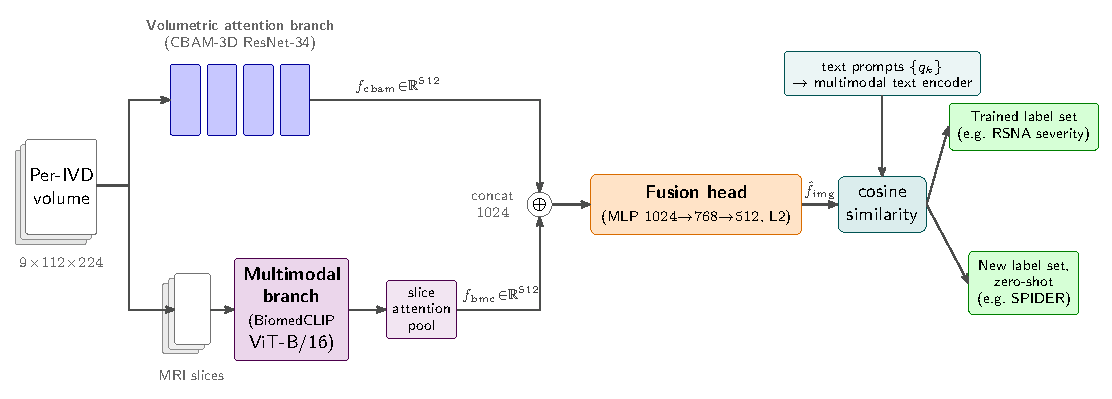
\includegraphics[width=\linewidth]{hybrid_arch_generic.pdf}
\caption{Two-branch hybrid architecture. A frozen volumetric attention branch and a frozen multimodal branch encode each per-IVD volume; a small MLP fuses their embeddings into a text-aligned vector scored by cosine similarity against text prompts, so the label set, whether a trained set or a new one (zero-shot), becomes an input at inference. Only the fusion MLP, slice-attention pool, scalar logit scale, and per-task uncertainty scalars are trained.}
\label{fig:arch}
\end{figure}

\subsection{Training Objective and Class-Imbalance Strategy}\label{sec:objective}

We handle class imbalance with a strategy that acts at three points: the loss, the gradient weighting, and the sampler.

The per-task loss is the focal cross-entropy~\cite{lin2017focal},
\begin{equation}
\mathrm{FL}_t(p_t) = -w_{y_t}\,(1 - p_t)^{\gamma}\, \log(p_t),
\label{eq:focal}
\end{equation}
where $p_t$ is the predicted probability of the ground-truth class $y_t$ and $w_{y_t}$ its class weight. We set $\gamma=1.8$ for CBAM-only and $\gamma=2.0$ for Multimodal-only and Hybrid; the factor $(1 - p_t)^{\gamma}$ down-weights easy samples so the gradient concentrates on hard minority cases. For the Multimodal-only and Hybrid configurations the focal loss is applied to the cosine logits of Eq.~\ref{eq:cosinehead} rather than to logits from a linear head, and we add a per-task supervised-contrastive term~\cite{khosla2020supcon} on the resulting image embeddings (weight $\lambda=0.1$, temperature $0.07$) that pulls same-class embeddings together; missing labels are excluded from both the focal and contrastive terms. The per-task losses are then combined by learned homoscedastic-uncertainty weighting~\cite{kendall2018multitask} rather than a plain sum.

Class weighting controls the gradient magnitude per class: we set $w_c \propto 1/\sqrt{n_c}$, normalized to mean one over the class counts $n_c$. The square root softens the imbalance, reducing the Severe-to-Normal gradient ratio from about $15\times$ under linear $1/n_c$ weighting to about $4\times$. Minority oversampling (factor 3 to 5) then changes how often a Severe sample is seen, while $w_c$ reweights its gradient in the batch. Augmentation adds geometric and intensity transforms; the exact transforms and all hyperparameters are given in Section~\ref{exp1}.

%==============================================%
\section{Experiments and Analysis}\label{sec4}

\subsection{Experimental Setup}\label{exp1}

Our method is dataset-agnostic; here we instantiate the source schema with RSNA 2024~\cite{kaggle2024} and the target schema with SPIDER~\cite{vandergraaf2024spider} (Table~\ref{tab:datasets}). RSNA supplies training and in-domain evaluation (patient-level 80/20 split), and the full SPIDER cohort is held out for cross-dataset transfer; only the supervised-transfer split (Section~\ref{sec:spider_transfer}) uses a smaller 34-patient validation. On RSNA we grade the three conditions suited to sagittal input (canal stenosis, left/right neural foraminal narrowing), leaving the two subarticular conditions, best read on axial reformats, to future work; the per-condition severity split is heavily skewed toward Normal/Mild, with Severe $\approx 5\%$ (Figure~\ref{fig:dist}). For SPIDER we use the T2-FS series only (excluding the T1 scans) for consistency with the RSNA-trained encoder; its eight labels (Pfirrmann 1--5~\cite{pfirrmann2001}, Modic 0--3~\cite{modic1988}, and six binary findings) follow a different schema, and no SPIDER image is seen during RSNA training. Furthermore, Figure~\ref{fig:dist} reports the class distribution of both datasets: the RSNA Severe class stays under 5\%, and several SPIDER labels are similarly skewed. This imbalance is the central difficulty the training pipeline must handle.

\begin{table}[htbp]
\centering
\caption{Datasets used. RSNA 2024 is the training and in-domain set; SPIDER is held out for cross-dataset transfer (T2-FS series only).}
\label{tab:datasets}
\footnotesize
\begin{tabular}{@{}llll@{}}
\toprule
\textbf{Dataset} & \textbf{Patients} & \textbf{Validation IVDs} & \textbf{Sequence} \\
\midrule
RSNA 2024 & $\sim$2{,}000 & 1{,}942 (395 patients) & sagittal T2 \\
SPIDER & 218 & 1{,}439 (208 patients) & sagittal T2-FS \\
\bottomrule
\end{tabular}
\end{table}

\begin{figure}[ht]
\centering
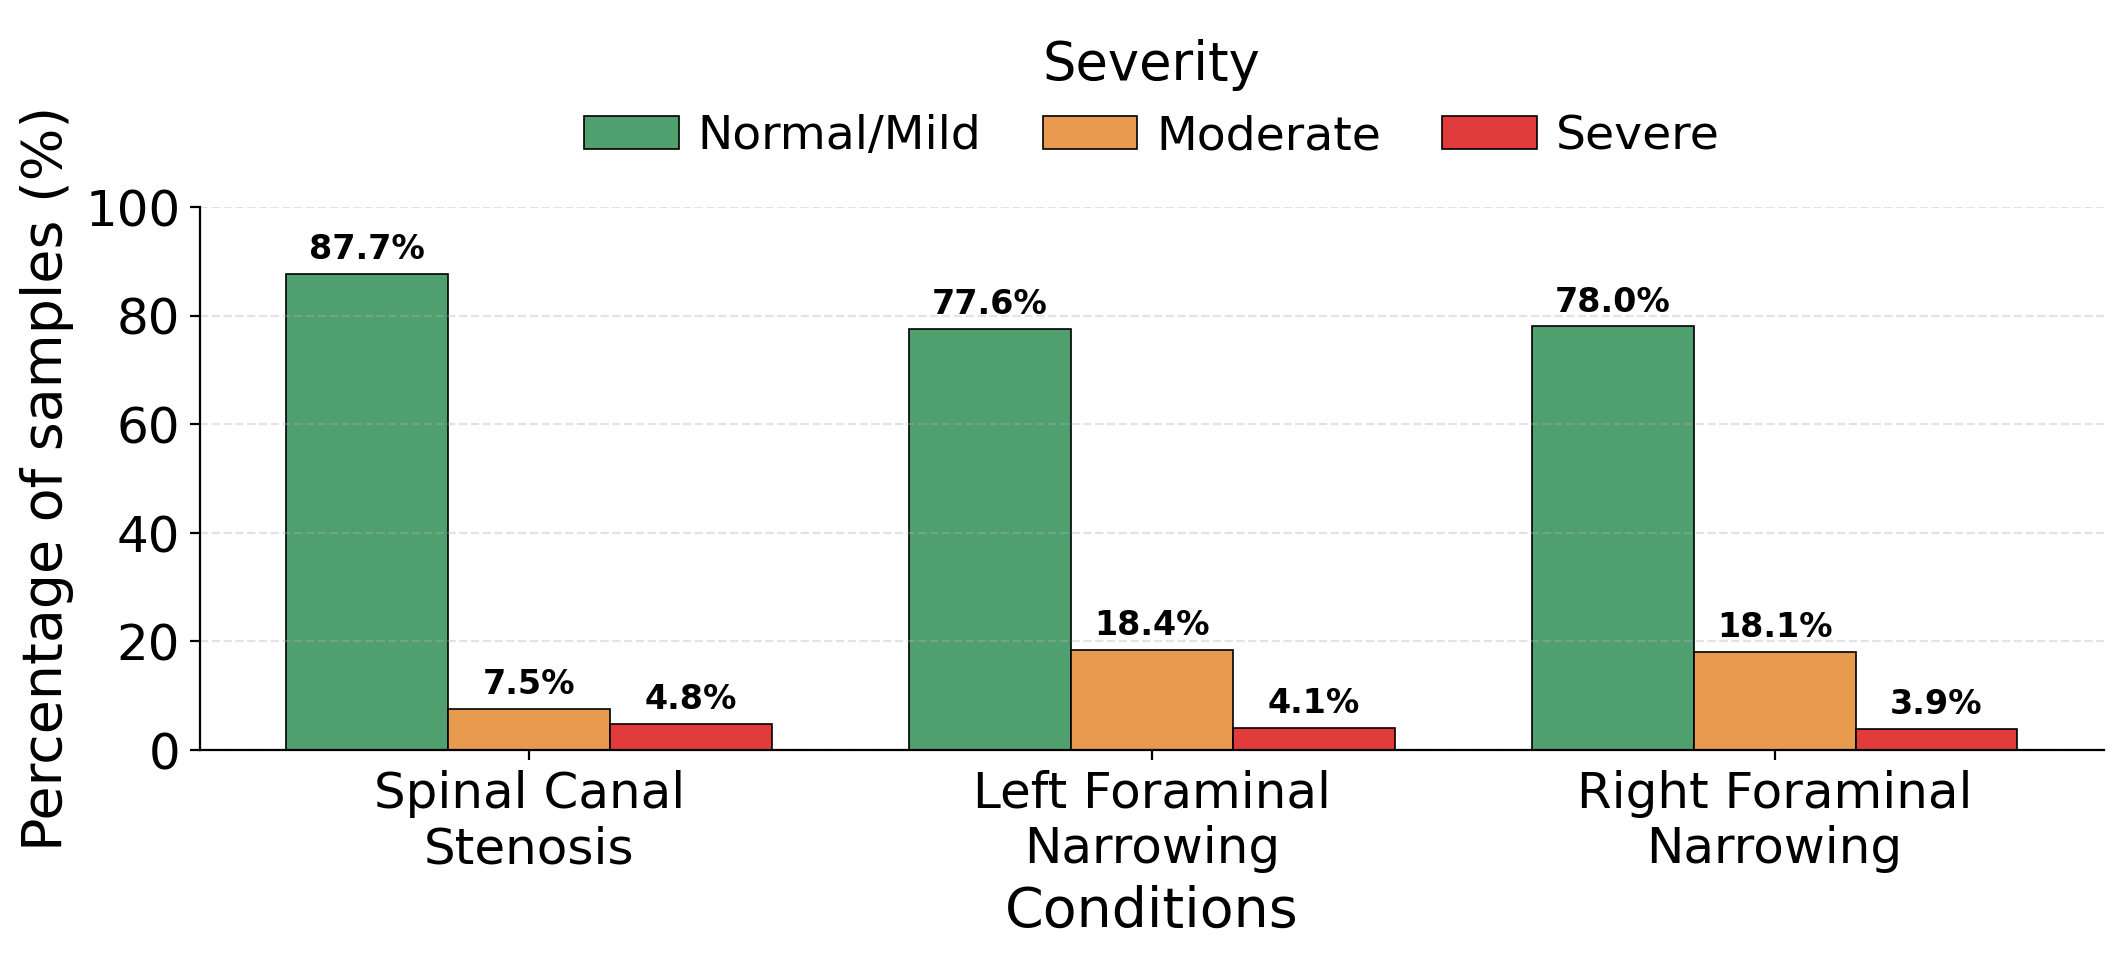
\includegraphics[width=0.82\linewidth]{rsna_class_distribution_en.png}\\[2pt]
{\small (a) RSNA 2024}\\[6pt]
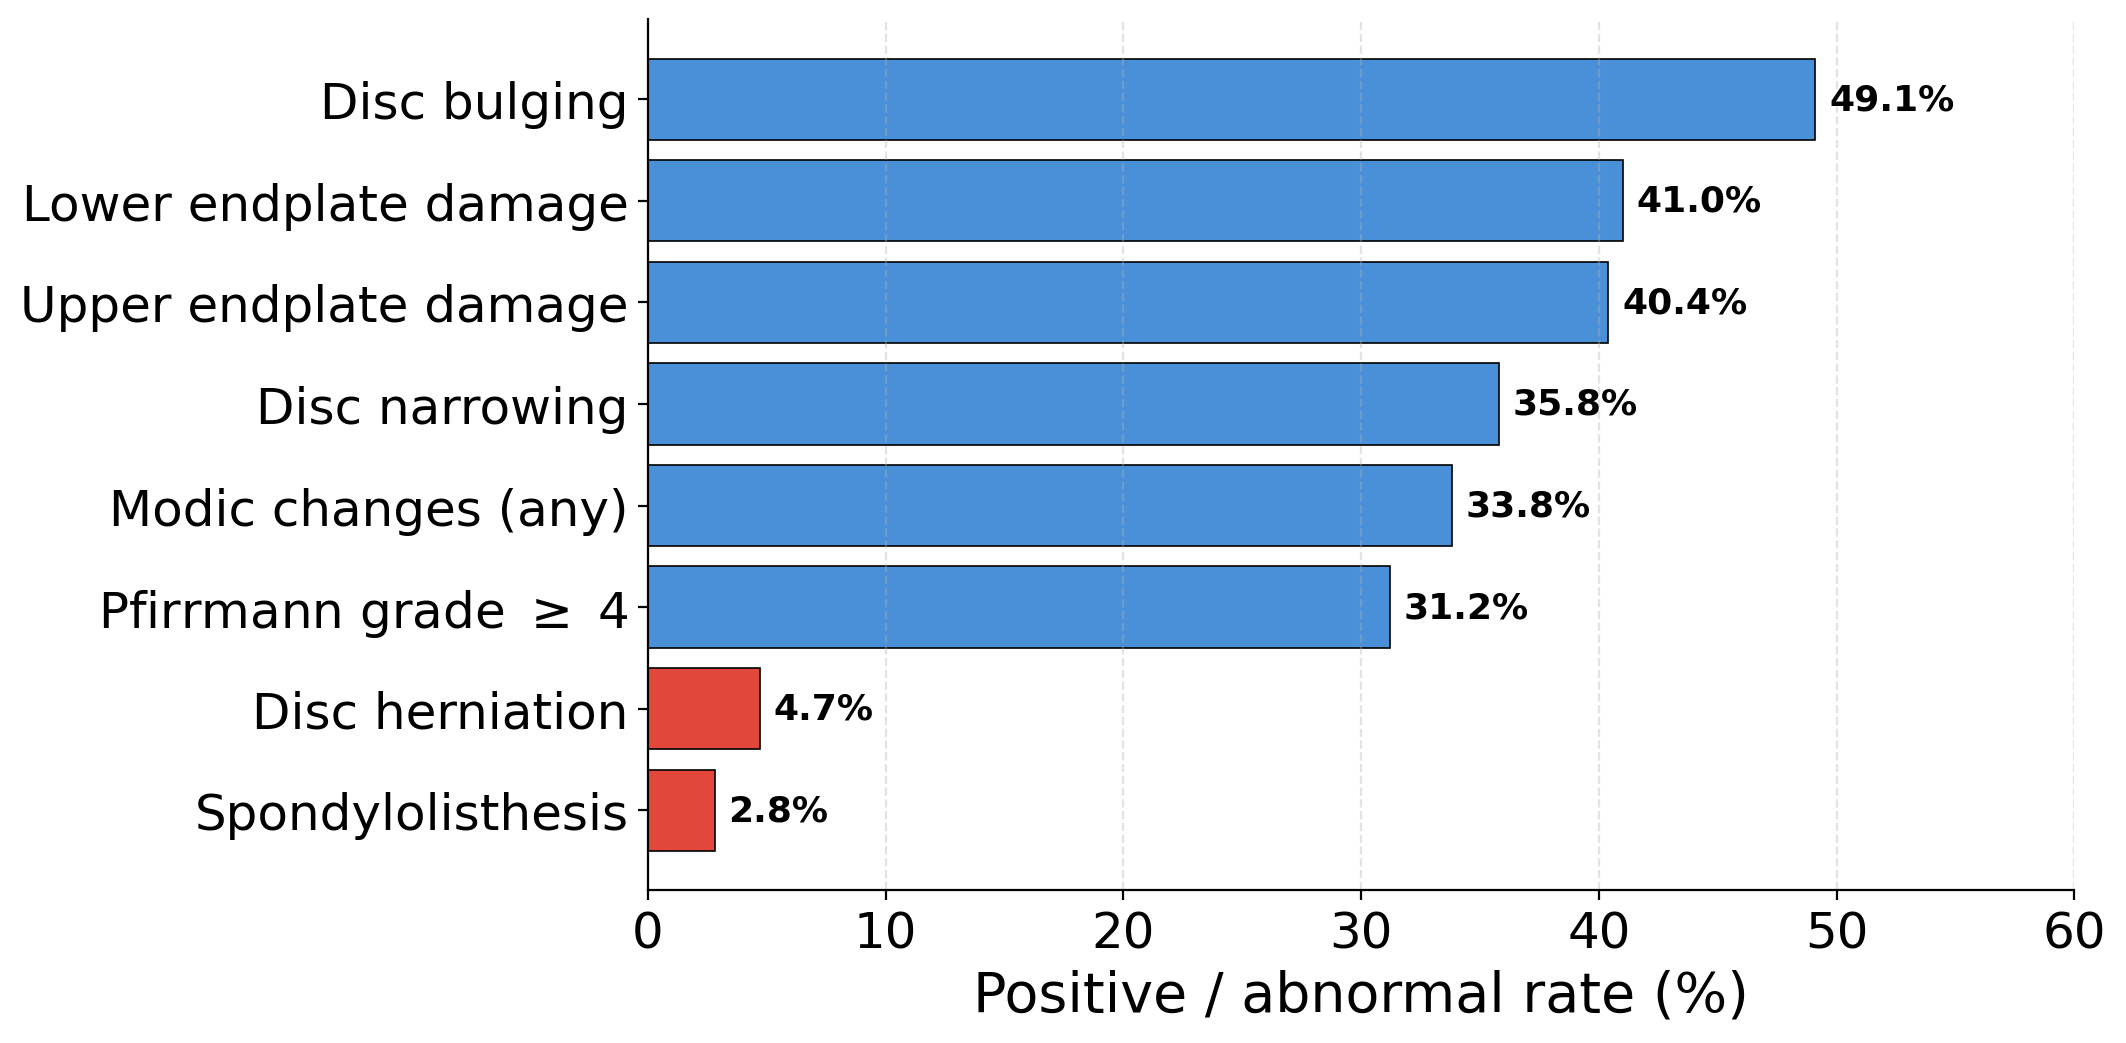
\includegraphics[width=0.82\linewidth]{spider_class_distribution_en.png}\\[2pt]
{\small (b) SPIDER}\\[4pt]
\caption{Class distribution of the two datasets. (a) RSNA 2024 per-condition severity, where Normal/Mild dominates and Severe stays under 5\%. (b) SPIDER eight-label distribution, where several pathology labels are heavily skewed toward the negative class.}
\label{fig:dist}
\end{figure}

We compare four configurations sharing the same 3D ResNet-34 backbone and per-IVD input: \emph{SpineNetV2}, denoting the reused 3D ResNet-34 grading backbone of~\cite{windsor2022} (not the full official pipeline); \emph{CBAM-only}, that backbone with channel-spatial attention; \emph{Multimodal-only}, the frozen multimodal branch (BiomedCLIP) alone; and the full \emph{Hybrid} (our proposed model). This lets us separate each branch's contribution.

For evaluation we report macro-averaged Recall, Precision, F1, AUC (one-vs-rest), and AUPRC, plus per-class Severe metrics. Macro averaging over the $C=3$ severities keeps the dominant Normal/Mild class from masking Severe failure; we add AUPRC because AUC can stay high on imbalanced data while a model still fails to rank Severe cases. Moreover, we form one volumetric crop per disc (L1--L2 through L5--S1) from the keypoint annotations, clip intensities to the 1st--99th percentile, and rescale to $[0,1]$. Table~\ref{tab:config} summarizes the training configuration.

\begin{table}[t]
\centering
\caption{Training configuration. Both backbones stay frozen; only the fusion MLP, slice-attention pool, scalar logit scale, and per-task uncertainty scalars are trained.}
\label{tab:config}
\footnotesize
\begin{tabular}{@{}l p{8.1cm}@{}}
\toprule
\textbf{Setting} & \textbf{Value} \\
\midrule
Per-IVD input & $1\times9\times112\times224$ tensor; embedding dim $d=512$ \\
Trainable / total params & 1.18\,M / 260\,M \\
Optimizer & AdamW, lr $10^{-4}$, weight decay $10^{-4}$ \\
Batch / epochs & 32 / $\leq$20, early stopping (patience 5) \\
Augmentation & h-flip + L/R swap, rotate $\pm10^{\circ}$, bright./contrast $\pm20\%$, noise $\sigma{=}0.05$ ($p{=}0.3$) \\
Hardware & 1$\times$ NVIDIA RTX 4090 ($\approx$16\,GB) \\
\bottomrule
\end{tabular}
\end{table}

\subsection{In-Domain Results and Ablation on RSNA 2024}\label{exp2}

Table~\ref{tab:main} reports ten metrics on the RSNA 2024 validation split (mean $\pm$ std over three seeds) for the four configurations. The Hybrid wins on every metric except Mean Accuracy, which we explain below.

\begin{table}[htbp]
\centering
\caption{Ablation on RSNA 2024 validation (1{,}942 IVDs / 395 patients), mean $\pm$ std over 3 seeds \{42, 123, 456\}. \textbf{Bold} = best per row; Mean Accuracy is secondary under imbalance.}
\label{tab:main}
\footnotesize
\setlength{\tabcolsep}{2pt}
\begin{tabular}{@{}lcccc@{}}
\toprule
\textbf{Metric} & \textbf{SpineNetV2} & \textbf{CBAM-only} & \textbf{Multimodal-only} & \textbf{Hybrid (Ours)} \\
\midrule
Mean Accuracy        & \best{81.0 $\pm$ 0.6} & 69.5 $\pm$ 1.0 & 71.2 $\pm$ 1.7 & 72.4 $\pm$ 0.3 \\
Mean F1 macro        & 0.420 $\pm$ 0.010 & 0.477 $\pm$ 0.057 & 0.482 $\pm$ 0.019 & \best{0.527 $\pm$ 0.027} \\
Mean Recall macro    & 0.412 $\pm$ 0.005 & 0.531 $\pm$ 0.068 & 0.532 $\pm$ 0.004 & \best{0.592 $\pm$ 0.026} \\
Mean Precision macro & 0.493 $\pm$ 0.028 & 0.499 $\pm$ 0.037 & 0.508 $\pm$ 0.037 & \best{0.526 $\pm$ 0.013} \\
Mean AUC macro       & 0.835 $\pm$ 0.010 & 0.803 $\pm$ 0.050 & 0.826 $\pm$ 0.015 & \best{0.838 $\pm$ 0.018} \\
Mean AUPRC macro     & 0.530 $\pm$ 0.012 & 0.498 $\pm$ 0.051 & 0.513 $\pm$ 0.030 & \best{0.533 $\pm$ 0.024} \\
\midrule
\textbf{Severe Recall} & 0.123 $\pm$ 0.005 & 0.288 $\pm$ 0.092 & 0.316 $\pm$ 0.042 & \best{0.486 $\pm$ 0.016} \\
\textbf{Severe F1}    & 0.152 $\pm$ 0.008 & 0.262 $\pm$ 0.082 & 0.268 $\pm$ 0.034 & \best{0.356 $\pm$ 0.017} \\
\textbf{Severe AUC}   & 0.872 $\pm$ 0.011 & 0.865 $\pm$ 0.050 & 0.885 $\pm$ 0.010 & \best{0.899 $\pm$ 0.011} \\
\textbf{Severe AUPRC} & 0.284 $\pm$ 0.019 & 0.278 $\pm$ 0.099 & 0.275 $\pm$ 0.052 & \best{0.333 $\pm$ 0.042} \\
\bottomrule
\end{tabular}
\end{table}

The Hybrid's F1 (0.527) exceeds both single branches (CBAM-only 0.477, Multimodal-only 0.482) by $0.045$ to $0.050$ in absolute macro-F1, so the two sources add information rather than duplicate it. Meanwhile, the largest gains are on the Severe class. Severe F1 rises 2.3$\times$ (0.152 to 0.356), Severe Recall about 4$\times$ (12.3\% to 48.6\%), and Severe AUC to 0.899; the Severe AUPRC of 0.333 against the $\approx$0.05 prevalence baseline is a 6.7$\times$ gain over chance. The 8.6-point Mean Accuracy drop is the cost of rebalancing: SpineNetV2 scores high accuracy mainly by predicting Normal/Mild everywhere, so the hybrid trades majority-class accuracy for minority-class recall.

\subsection{Cross-Dataset Zero-Shot Transfer to SPIDER}

Published work on SPIDER is mostly segmentation~\cite{vandergraaf2024spider}; we are not aware of prior reports of cross-dataset zero-shot transfer (RSNA to SPIDER) via text-prompt label-space extension. We freeze the RSNA-trained hybrid and score the eight SPIDER categories by cosine similarity against fixed prompts (``a magnetic resonance image of \emph{[label]}'', e.g.\ ``lumbar disc herniation'' vs.\ ``no disc herniation''), written a priori, so no target-label leakage occurs and no SPIDER data is used. Over the full cohort (1{,}439 IVDs, 208 patients) the hybrid reaches mean F1 = 0.362 across the eight unseen labels (Table~\ref{tab:spider}), which fixed-head baselines cannot do without retraining.

\begin{table}[htbp]
\centering
\caption{Zero-shot transfer to SPIDER (macro-F1, no fine-tuning), recomputed from cosine predictions. \emph{Off-the-shelf} = BiomedCLIP scored zero-shot with no RSNA training; \emph{Hybrid} = our RSNA-trained model. \textbf{Bold} = higher F1.}
\label{tab:spider}
\begin{tabular}{@{}lcc@{}}
\toprule
\textbf{SPIDER label}              & \textbf{Off-the-shelf} & \textbf{Hybrid (Ours)} \\
\midrule
Disc bulging              & 0.363 & \best{0.613} \\
Disc herniation           & 0.532 & \best{0.563} \\
Disc narrowing            & 0.403 & \best{0.586} \\
\midrule
Upper endplate            & \best{0.569} & 0.467 \\
Lower endplate            & \best{0.558} & 0.468 \\
Pfirrmann (5-class)       & 0.152 & \best{0.155} \\
Modic (4-class)           & \best{0.071} & 0.018 \\
Spondylolisthesis         & \best{0.500} & 0.028 \\
\midrule
Mean (disc-morphology)    & 0.433 & \best{0.587} \\
Mean (all 8)              & \best{0.394} & 0.362 \\
\bottomrule
\end{tabular}
\end{table}

Transfer is uneven across labels. On the three disc-morphology labels closest to the RSNA schema (bulging, herniation, narrowing) the RSNA-trained hybrid clearly beats the off-the-shelf BiomedCLIP baseline (Table~\ref{tab:spider}); on labels far from that schema (endplate, spondylolisthesis) the baseline is competitive or better, so its all-eight mean F1 (0.394) edges the hybrid (0.362). RSNA supervision therefore improves zero-shot transfer mainly for semantically related disc-morphology labels, not uniformly across all target labels. The weakest label is Modic (F1 0.018): a task-input limit rather than a model one, since SPIDER's T2-FS lacks the paired T1 sequence Modic grading needs.

\subsection{Supervised Transfer on the SPIDER 8-Label Schema}
\label{sec:spider_transfer}

To assess transfer beyond zero-shot, we train on the SPIDER training split for 15 epochs with the image backbones frozen: SpineNetV2 and CBAM-only fit lightweight task-specific linear heads, while Multimodal-only and Hybrid keep cosine scoring against SPIDER text anchors and update only the trainable projection, slice-attention pool, and logit scale. We use across all four configurations and the full 8-label schema (Pfirrmann 5-class, Modic 4-class, six binary labels); Table~\ref{tab:spider_transfer_agg} reports the aggregate results. The 8-label set is split 80/20 at patient level (939 training / 234 validation IVDs); backbone parameters stay frozen for a fair comparison, and only the condition-specific heads (and the fusion MLP for Hybrid and Multimodal-only) are trained.

\begin{table}[htbp]
\centering
\caption{SPIDER transfer learning, four configurations, mean across 8 conditions on validation (234 IVDs), reported as mean $\pm$ standard deviation over 3 seeds $\{42, 123, 456\}$. \textbf{Bold} = best per row; inference is within seed noise. $^\ast$ = exploratory gain over CBAM ($n=3$ seeds); Hybrid vs.\ SpineNetV2 is statistical parity ($p=0.57$, footnote).}
\label{tab:spider_transfer_agg}
\footnotesize
\begin{tabular}{@{}lcccc@{}}
\toprule
\textbf{Metric} & \textbf{SpineNetV2} & \textbf{CBAM-only} & \textbf{Multimodal-only} & \textbf{Hybrid (Ours)} \\
\midrule
Mean Accuracy & \best{80.23 $\pm$ 0.94} & 79.27 $\pm$ 1.19 & 76.12 $\pm$ 0.83 & 78.30 $\pm$ 1.64 \\
Mean F1 macro & 0.646 $\pm$ 0.002 & 0.619 $\pm$ 0.010 & 0.613 $\pm$ 0.006 & \best{0.653 $\pm$ 0.014}$^\ast$ \\
Mean AUC      & 0.842 $\pm$ 0.006 & 0.824 $\pm$ 0.018 & 0.808 $\pm$ 0.011 & \best{0.846 $\pm$ 0.018}$^\ast$ \\
Mean AUPRC    & \best{0.633 $\pm$ 0.026} & 0.580 $\pm$ 0.016 & 0.544 $\pm$ 0.007 & 0.611 $\pm$ 0.010 \\
\midrule
Inference (ms/IVD) & 65.5 $\pm$ 2.7 & 66.7 $\pm$ 3.2 & 65.2 $\pm$ 3.9 & 66.4 $\pm$ 3.7 \\
\bottomrule
\end{tabular}

\vspace{2pt}
{\raggedright\scriptsize
$^\ast$Exploratory paired $t$-test over three seeds (per-seed Mean F1, Hybrid: 0.660/0.665/0.633, CBAM: 0.621/0.630/0.606): Hybrid vs.\ CBAM gives $\Delta=+0.034$ ($p=0.011$, 95\% CI $[0.018,0.049]$), Hybrid vs.\ SpineNetV2 is parity ($p=0.57$); with only three seeds we treat these as exploratory rather than confirmatory.\par}
\end{table}

We make two observations. The hybrid and SpineNetV2 are at parity on aggregate SPIDER metrics (F1 gap $+0.007$, within seed noise; SpineNetV2 even leads on AUPRC), so we do not claim the hybrid surpasses it. More telling, CBAM-only drops clearly below plain SpineNetV2 on transfer (Mean F1 $0.619$ vs.\ $0.646$, several times the inter-seed std) while the hybrid recovers above CBAM by $+0.034$ ($p=0.011$, exploratory at three seeds); we analyze this asymmetry in Section~\ref{sec:disc}.

The aggregate gains concentrate in the rare positive classes ($\leq 5\%$). On Disc Herniation, SpineNetV2 and CBAM recall no positive case ($0\%$) while Multimodal-only and the hybrid recover $27.0\%$ and $35.6\%$; the BiomedCLIP prior drives most of this, CBAM adding an incremental gain when fused. The same ordering holds for Spondylolisthesis and Pfirrmann Grade~4.

\subsection{Qualitative Results}

Figure~\ref{fig:gradcam} contrasts Grad-CAM~\cite{selvaraju2017gradcam} activation without and with CBAM on a representative Severe spinal-canal case. The maps are taken from the gradient of the Severe-class logit with respect to the last convolutional feature map and upsampled to the input resolution, so the brighter regions are the ones that pushed the Severe score up. Without attention the response is spread over most of the slice, including vertebral body and soft tissue well away from the canal. With CBAM it concentrates on the narrowed segment of the central canal, which is the region a radiologist reads for this label. This is qualitative support for the spatial-attention hypothesis and it agrees with the Severe gains in Table~\ref{tab:main}, although a saliency map only shows where the evidence sits and is not by itself proof of a mechanism.

The foraminal conditions behave differently. Severe recall settles lower there, between 18 and 22\%, well below the canal. This is the same ceiling that external validation of SpineNetV2 reports for sagittal-only foraminal reads~\cite{nigru2024}, which suggests the limit comes from what the input can show rather than from the attention block. Richer input for these two conditions is the natural next step and we leave it to future work.

\begin{figure}[htbp]
\centering

\includegraphics[width=0.8\linewidth]{grad_cam_nocbam_vs_cbam.png}
\caption{Grad-CAM (Severe-class logit, upsampled to input resolution) on a Severe spinal-canal case, without vs.\ with CBAM.}
\label{fig:gradcam}
\end{figure}

%==============================================%
\section{Discussion}\label{sec:disc}

We do not claim a new attention mechanism or a new vision-language pretraining method; our contribution is a controlled design study of how a frozen text-aligned biomedical prior changes the behavior of an attention-based volumetric grader under severe class imbalance and cross-dataset label shift. The attention branch both helps and hurts, depending on the dataset: in-domain both branches lift Severe F1 over SpineNetV2 to a similar degree (Table~\ref{tab:main}), but out-of-domain the attention-only model falls clearly below plain SpineNetV2 (Section~\ref{sec:spider_transfer}), consistent with overfitting RSNA-specific patterns, while the hybrid recovers to parity. We therefore read the frozen branch not as an additive gain over SpineNetV2 but as a regularizer: a reliable fallback when the attention branch's in-domain bias misaligns with the target (no mechanistic proof claimed). It is not a trivial ensemble either: averaging SpineNetV2 and Multimodal-only softmax outputs reaches only Mean F1 0.45 / Severe F1 0.18, well below the learned-fusion hybrid (0.53 / 0.36). Clinically, the Severe recall of 48.6\% (about 4$\times$ over baseline) is still below the $\approx$80\% sensitivity a screening tool needs, so the model is best used as a second-reader assistant that flags candidate Severe cases rather than as a standalone tool.

A few limitations remain. The regularization claim rests on a cross-dataset behavioral pattern, and a mechanistic account is left to future work. With only three seeds the reported $p$-values are exploratory, and the supervised-transfer validation is small (34 patients), although the zero-shot transfer is evaluated on the full SPIDER cohort (208 patients). The multimodal branch is also frozen and 2D, native-3D medical vision-language models remain an emerging direction we leave to future backbones, and the fusion is restricted to a concat-MLP. Finally, RSNA Severe inter-rater agreement was not released~\cite{kaggle2024}, so the Severe ceiling reflects label noise as well as model capacity. The fused embedding is aligned to text only through the RSNA source anchors it is trained against, with no additional image-text contrastive objective, so compatibility with unseen prompts is partial (stronger near the RSNA schema, Table~\ref{tab:spider}); a dedicated alignment loss and prompt-robustness study are left to future work. At inference both frozen backbones still run ($\approx$66\,ms/IVD): parameter-efficient to train, not lightweight to deploy.

%==============================================%
\section{Summary}\label{sec5}

We presented a two-branch model pairing volumetric attention with a frozen biomedical foundation encoder for lumbar IVD grading. Relative to a standard cross-entropy baseline, the full pipeline markedly improves the minority Severe class (Recall $\sim$4$\times$, F1 2.3$\times$, AUC 0.899) at a controlled accuracy trade-off, and extends zero-shot to eight unseen SPIDER labels without retraining. On cross-dataset transfer, attention alone drops F1 below plain SpineNetV2 while the frozen branch restores it, which we read as cross-dataset regularization. Future work includes a mechanistic representation analysis, a learned slice-pooling adapter~\cite{lu2024radclip}, and axial-T2 fusion.

% ----- Acknowledgments removed for double-blind review; restore for camera-ready -----
\begin{credits}
\subsubsection{\ackname} We acknowledge Ho Chi Minh City University of Technology (HCMUT), VNU-HCM for supporting this study.
\subsubsection{\discintname} The authors have no competing interests to declare that are relevant to the content of this article.
\end{credits}
%
\bibliographystyle{splncs04}
\bibliography{references}

\end{document}
